\documentclass{article}

\usepackage[utf8]{inputenc}
\usepackage[T1]{fontenc}
\usepackage{bm}

\usepackage{Sweave}
\begin{document}
\Sconcordance{concordance:aproximacao_polinomial.tex:aproximacao_polinomial.Rnw:%
1 6 1 1 0 10 1 1 3 1 0 1 1 1 2 2 1 1 2 1 1 1 2 2 1 3 0 1 2 5 1 1 3 1 0 %
1 2 3 1 1 2 3 1 1 3 1 0 1 1 1 2 3 1 4 0 1 2 3 1 1 3 1 0 1 2 3 1 1 2 3 1 %
1 3 1 0 1 1 1 2 3 1 4 0 1 2 3 1 1 3 1 0 1 2 3 1 1 2 3 1 1 3 1 0 1 1 1 2 %
3 1 4 0 1 2 3 1 1 3 1 0 1 2 3 1 1 2 3 1 1 3 1 0 1 1 1 2 3 1 4 0 1 2 3 1 %
1 3 1 0 1 2 3 1 1 2 3 1 1 3 1 0 1 1 1 2 3 1 4 0 1 2 3 1 1 3 1 0 1 2 3 1 %
1 2 3 1 1 3 1 0 1 1 1 2 3 1 4 0 1 2 3 1 1 3 1 0 1 2 3 1 1 2 3 1 1 3 1 0 %
1 1 1 2 3 1 4 0 1 2 3 1 1 3 1 0 1 2 3 1 1 2 3 1 1 3 1 0 1 1 1 2 3 1 4 0 %
1 2 13 1 1 3 1 0 1 2 3 1 1 2 3 1 1 3 1 0 1 1 1 2 3 1 4 0 1 2 3 1 1 3 1 %
0 1 2 3 1 1 2 3 1 1 3 1 0 1 1 1 2 3 1 4 0 1 2 3 1 1 3 1 0 1 2 3 1 1 2 3 %
1 1 3 1 0 1 1 1 2 3 1 4 0 1 2 3 1 1 3 1 0 1 2 3 1 1 2 3 1 1 3 1 0 1 1 1 %
2 3 1 4 0 1 2 3 1 1 3 1 0 1 2 3 1 1 2 3 1 1 3 1 0 1 1 1 2 3 1 4 0 1 2 3 %
1 1 3 1 0 1 2 3 1 1 2 3 1 1 3 1 0 1 1 1 2 3 1 4 0 1 2 3 1 1 3 1 0 1 2 3 %
1 1 2 3 1 1 3 1 0 1 1 1 2 3 1 4 0 1 2 3 1 1 3 1 0 1 2 3 1 1 2 3 1 1 3 1 %
0 1 1 1 2 3 1 4 0 1 2 13 1}


\title{Aproximação Polinomial}
\author{Matheus Araujo - 2013066265}
\date{}

\maketitle

Parametrização:

\begin{Schunk}
\begin{Sinput}
>   rm(list=ls())
>   library('corpcor')
>   xmin<--15
>   xmax<-10
>   xstep<-0.1
>   ymin<-0
>   ymax<-100
>   a1<-0.5
>   a2<-3
>   a3<-10
\end{Sinput}
\end{Schunk}

\newpage
\section{Aproximação Polinomial - 10 amostras}

\subsection{Polinômio Grau 1 - 10 amostras}

\begin{Schunk}
\begin{Sinput}
>   N<-10
>   x<-runif(n=N, min=xmin,max=xmax)
>   xgrid<-seq(xmin,xmax,xstep)
>   yr<-(a1*x^2+a2*x+a3)+rnorm(length(x))
>   ygrid<-(a1*xgrid^2+a2*xgrid+a3)
>   plot(x,yr,col='red',type='p', xlim=c(xmin,xmax), ylim=c(ymin,ymax),xlab='',ylab='')
>   par(new=T)
>   plot(xgrid,ygrid,col='gray',type='l', xlim=c(xmin,xmax), ylim=c(ymin,ymax),xlab='',ylab='')
>   par(new=T)
>   #aproximacao de grau 1
>   H<-cbind(x,1)
>   w<-pseudoinverse(H) %*% yr
>   Hgrid<-cbind(xgrid,1)
>   yhat<-H%*%w
>   yhatgrid<-Hgrid%*%w
>   plot(xgrid,yhatgrid,col='blue',type='l', xlim=c(xmin,xmax), ylim=c(ymin,ymax),xlab='x',ylab='y')
\end{Sinput}
\end{Schunk}
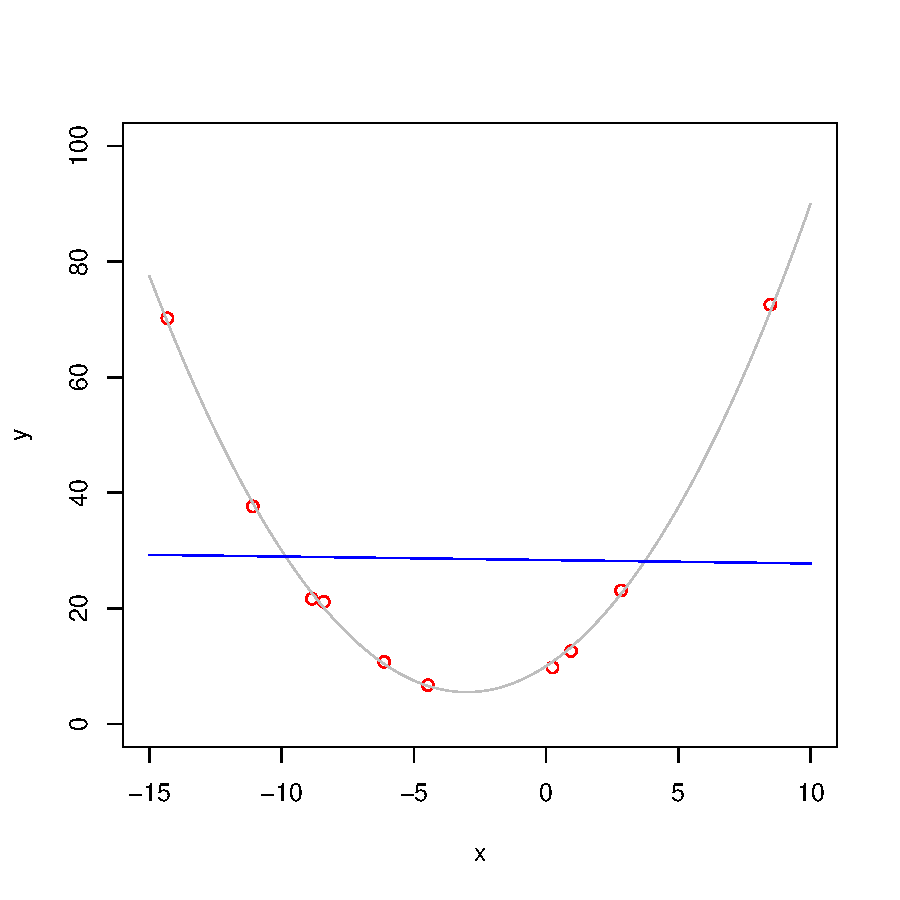
\includegraphics{aproximacao_polinomial-002}

\newpage
\subsection{Polinômio Grau 2 - 10 amostras}

\begin{Schunk}
\begin{Sinput}
>   N<-10
>   x<-runif(n=N, min=xmin,max=xmax)
>   xgrid<-seq(xmin,xmax,xstep)
>   yr<-(a1*x^2+a2*x+a3)+rnorm(length(x))
>   ygrid<-(a1*xgrid^2+a2*xgrid+a3)
>   plot(x,yr,col='red',type='p', xlim=c(xmin,xmax), ylim=c(ymin,ymax),xlab='',ylab='')
>   par(new=T)
>   plot(xgrid,ygrid,col='gray',type='l', xlim=c(xmin,xmax), ylim=c(ymin,ymax),xlab='',ylab='')
>   par(new=T)
>   #aproximacao de grau 2
>   H<-cbind(x^2,x,1)
>   w<-pseudoinverse(H) %*% yr
>   Hgrid<-cbind(xgrid^2,xgrid,1)
>   yhat<-H%*%w
>   yhatgrid<-Hgrid%*%w
>   plot(xgrid,yhatgrid,col='blue',type='l', xlim=c(xmin,xmax), ylim=c(ymin,ymax),xlab='x',ylab='y')
\end{Sinput}
\end{Schunk}
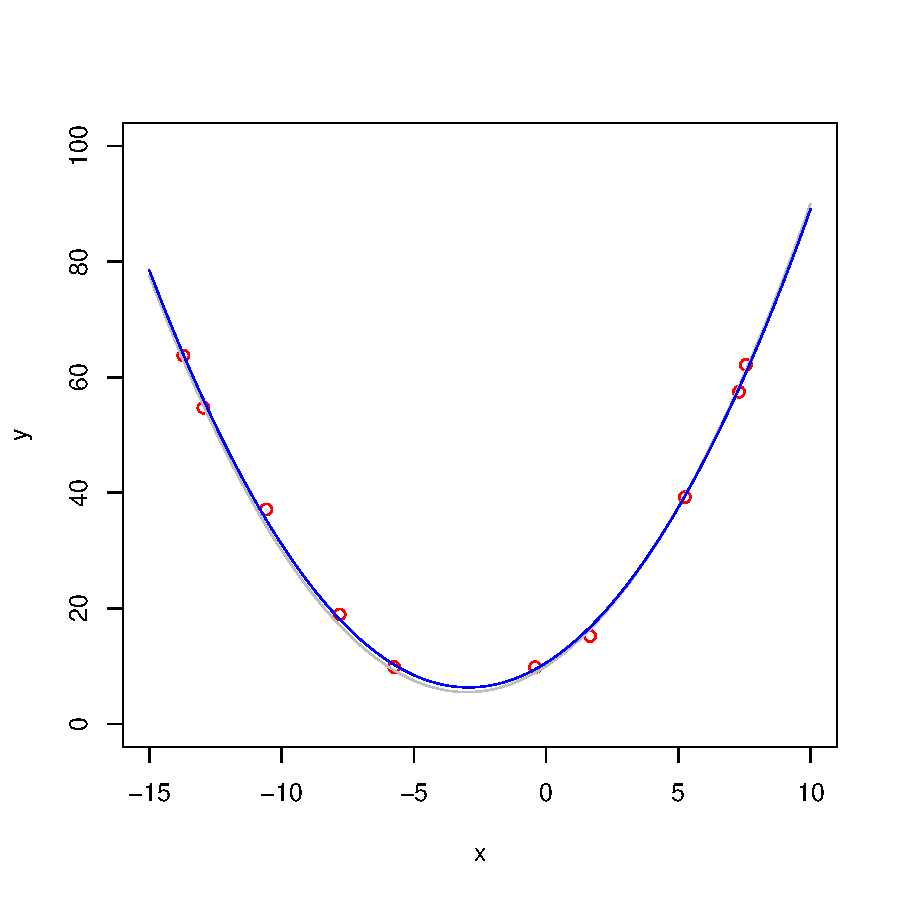
\includegraphics{aproximacao_polinomial-003}

\newpage
\subsection{Polinômio Grau 3 - 10 amostras}

\begin{Schunk}
\begin{Sinput}
>   N<-10
>   x<-runif(n=N, min=xmin,max=xmax)
>   xgrid<-seq(xmin,xmax,xstep)
>   yr<-(a1*x^2+a2*x+a3)+rnorm(length(x))
>   ygrid<-(a1*xgrid^2+a2*xgrid+a3)
>   plot(x,yr,col='red',type='p', xlim=c(xmin,xmax), ylim=c(ymin,ymax),xlab='',ylab='')
>   par(new=T)
>   plot(xgrid,ygrid,col='gray',type='l', xlim=c(xmin,xmax), ylim=c(ymin,ymax),xlab='',ylab='')
>   par(new=T)
>   #aproximacao de grau 3
>   H<-cbind(x^3,x^2,x,1)
>   w<-pseudoinverse(H) %*% yr
>   Hgrid<-cbind(xgrid^3,xgrid^2,xgrid,1)
>   yhat<-H%*%w
>   yhatgrid<-Hgrid%*%w
>   plot(xgrid,yhatgrid,col='blue',type='l', xlim=c(xmin,xmax), ylim=c(ymin,ymax),xlab='x',ylab='y')
\end{Sinput}
\end{Schunk}
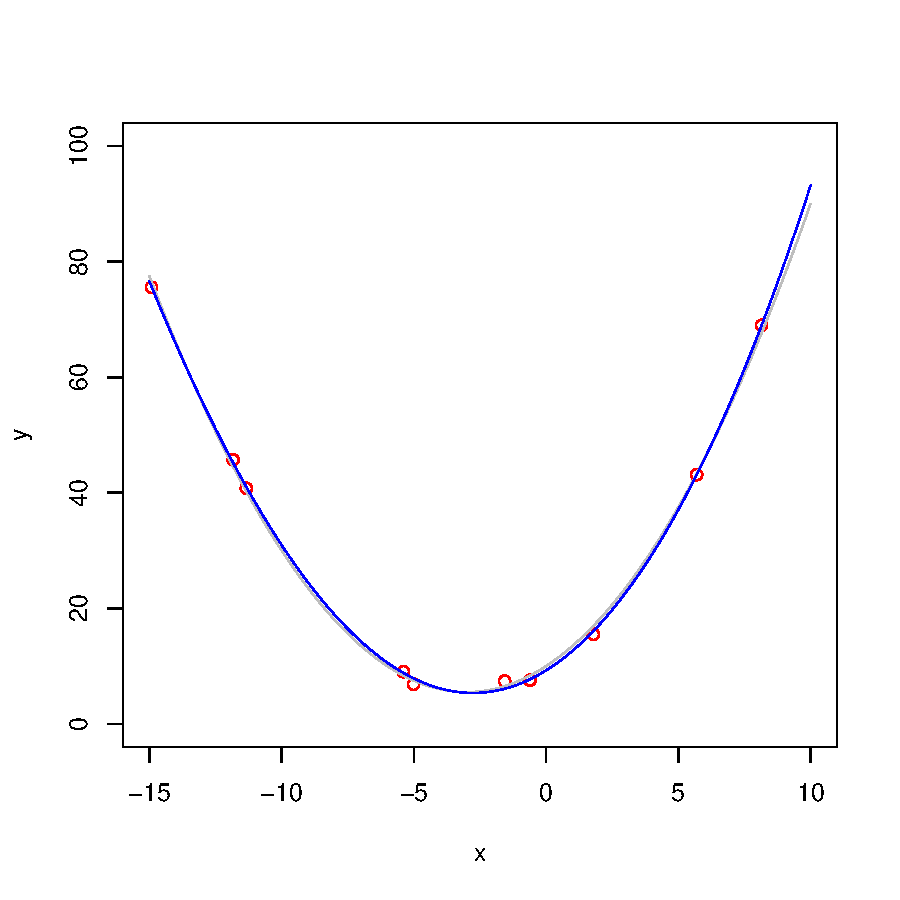
\includegraphics{aproximacao_polinomial-004}

\newpage
\subsection{Polinômio Grau 4 - 10 amostras}

\begin{Schunk}
\begin{Sinput}
>   N<-10
>   x<-runif(n=N, min=xmin,max=xmax)
>   xgrid<-seq(xmin,xmax,xstep)
>   yr<-(a1*x^2+a2*x+a3)+rnorm(length(x))
>   ygrid<-(a1*xgrid^2+a2*xgrid+a3)
>   plot(x,yr,col='red',type='p', xlim=c(xmin,xmax), ylim=c(ymin,ymax),xlab='',ylab='')
>   par(new=T)
>   plot(xgrid,ygrid,col='gray',type='l', xlim=c(xmin,xmax), ylim=c(ymin,ymax),xlab='',ylab='')
>   par(new=T)
>   #aproximacao de grau 4
>   H<-cbind(x^4,x^3,x^2,x,1)
>   w<-pseudoinverse(H) %*% yr
>   Hgrid<-cbind(xgrid^4,xgrid^3,xgrid^2,xgrid,1)
>   yhat<-H%*%w
>   yhatgrid<-Hgrid%*%w
>   plot(xgrid,yhatgrid,col='blue',type='l', xlim=c(xmin,xmax), ylim=c(ymin,ymax),xlab='x2',ylab='y2')
\end{Sinput}
\end{Schunk}
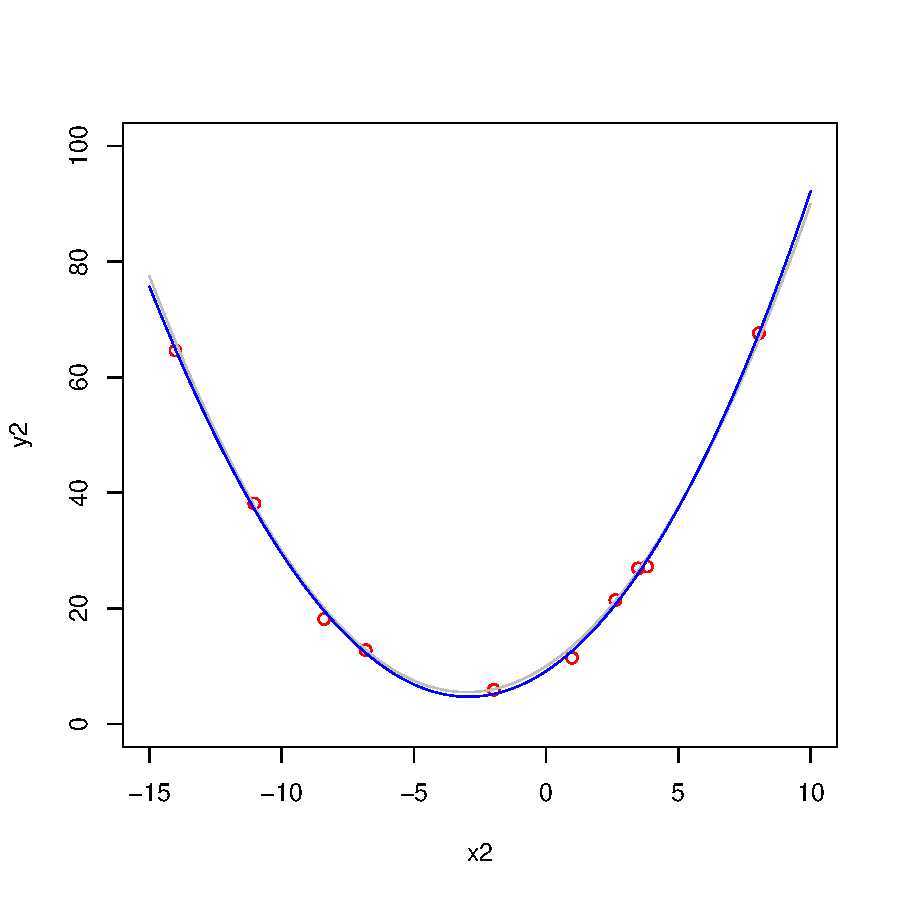
\includegraphics{aproximacao_polinomial-005}

\newpage
\subsection{Polinômio Grau 5 - 10 amostras}

\begin{Schunk}
\begin{Sinput}
>   N<-10
>   x<-runif(n=N, min=xmin,max=xmax)
>   xgrid<-seq(xmin,xmax,xstep)
>   yr<-(a1*x^2+a2*x+a3)+rnorm(length(x))
>   ygrid<-(a1*xgrid^2+a2*xgrid+a3)
>   plot(x,yr,col='red',type='p', xlim=c(xmin,xmax), ylim=c(ymin,ymax),xlab='',ylab='')
>   par(new=T)
>   plot(xgrid,ygrid,col='gray',type='l', xlim=c(xmin,xmax), ylim=c(ymin,ymax),xlab='',ylab='')
>   par(new=T)
>   #aproximacao de grau 5
>   H<-cbind(x^5,x^4,x^3,x^2,x,1)
>   w<-pseudoinverse(H) %*% yr
>   Hgrid<-cbind(xgrid^5,xgrid^4,xgrid^3,xgrid^2,xgrid,1)
>   yhat<-H%*%w
>   yhatgrid<-Hgrid%*%w
>   plot(xgrid,yhatgrid,col='blue',type='l', xlim=c(xmin,xmax), ylim=c(ymin,ymax),xlab='x2',ylab='y2')
\end{Sinput}
\end{Schunk}
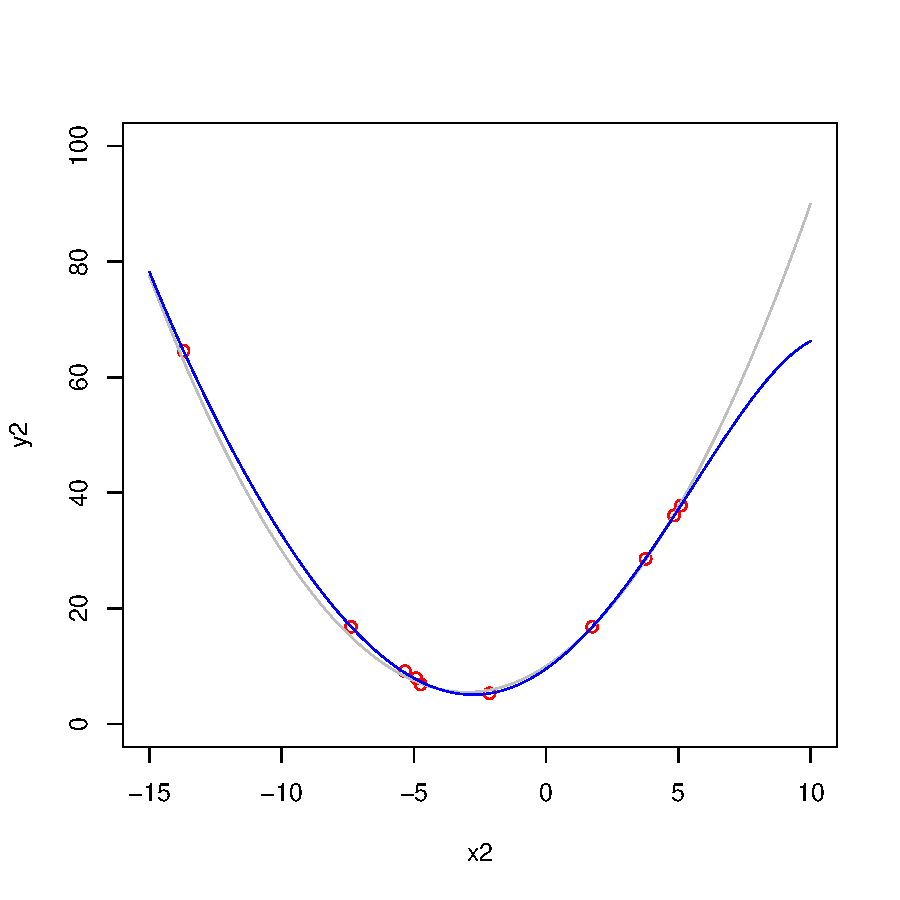
\includegraphics{aproximacao_polinomial-006}

\newpage
\subsection{Polinômio Grau 6 - 10 amostras}

\begin{Schunk}
\begin{Sinput}
>   N<-10
>   x<-runif(n=N, min=xmin,max=xmax)
>   xgrid<-seq(xmin,xmax,xstep)
>   yr<-(a1*x^2+a2*x+a3)+rnorm(length(x))
>   ygrid<-(a1*xgrid^2+a2*xgrid+a3)
>   plot(x,yr,col='red',type='p', xlim=c(xmin,xmax), ylim=c(ymin,ymax),xlab='',ylab='')
>   par(new=T)
>   plot(xgrid,ygrid,col='gray',type='l', xlim=c(xmin,xmax), ylim=c(ymin,ymax),xlab='',ylab='')
>   par(new=T)
>   #aproximacao de grau 6
>   H<-cbind(x^6,x^5,x^4,x^3,x^2,x,1)
>   w<-pseudoinverse(H) %*% yr
>   Hgrid<-cbind(xgrid^6,xgrid^5,xgrid^4,xgrid^3,xgrid^2,xgrid,1)
>   yhat<-H%*%w
>   yhatgrid<-Hgrid%*%w
>   plot(xgrid,yhatgrid,col='blue',type='l', xlim=c(xmin,xmax), ylim=c(ymin,ymax),xlab='x2',ylab='y2')
\end{Sinput}
\end{Schunk}
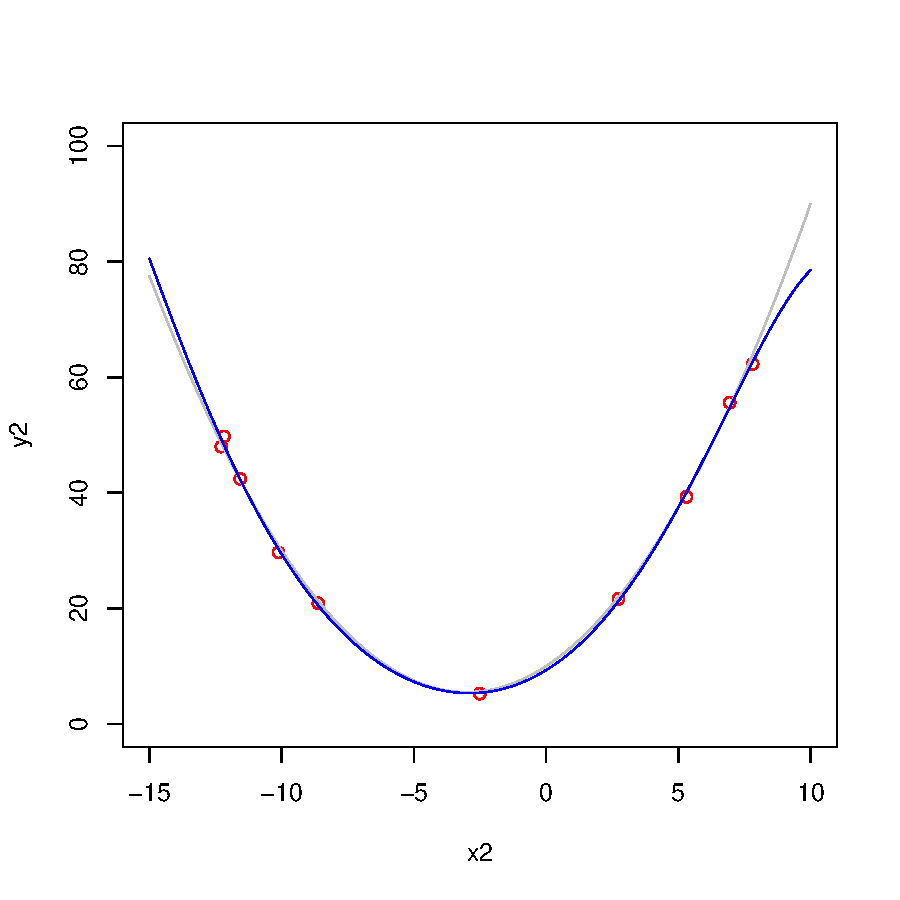
\includegraphics{aproximacao_polinomial-007}

\newpage
\subsection{Polinômio Grau 7 - 10 amostras}

\begin{Schunk}
\begin{Sinput}
>   N<-10
>   x<-runif(n=N, min=xmin,max=xmax)
>   xgrid<-seq(xmin,xmax,xstep)
>   yr<-(a1*x^2+a2*x+a3)+rnorm(length(x))
>   ygrid<-(a1*xgrid^2+a2*xgrid+a3)
>   plot(x,yr,col='red',type='p', xlim=c(xmin,xmax), ylim=c(ymin,ymax),xlab='',ylab='')
>   par(new=T)
>   plot(xgrid,ygrid,col='gray',type='l', xlim=c(xmin,xmax), ylim=c(ymin,ymax),xlab='',ylab='')
>   par(new=T)
>   #aproximacao de grau 7
>   H<-cbind(x^7,x^6,x^5,x^4,x^3,x^2,x,1)
>   w<-pseudoinverse(H) %*% yr
>   Hgrid<-cbind(xgrid^7,xgrid^6,xgrid^5,xgrid^4,xgrid^3,xgrid^2,xgrid,1)
>   yhat<-H%*%w
>   yhatgrid<-Hgrid%*%w
>   plot(xgrid,yhatgrid,col='blue',type='l', xlim=c(xmin,xmax), ylim=c(ymin,ymax),xlab='x2',ylab='y2')
\end{Sinput}
\end{Schunk}
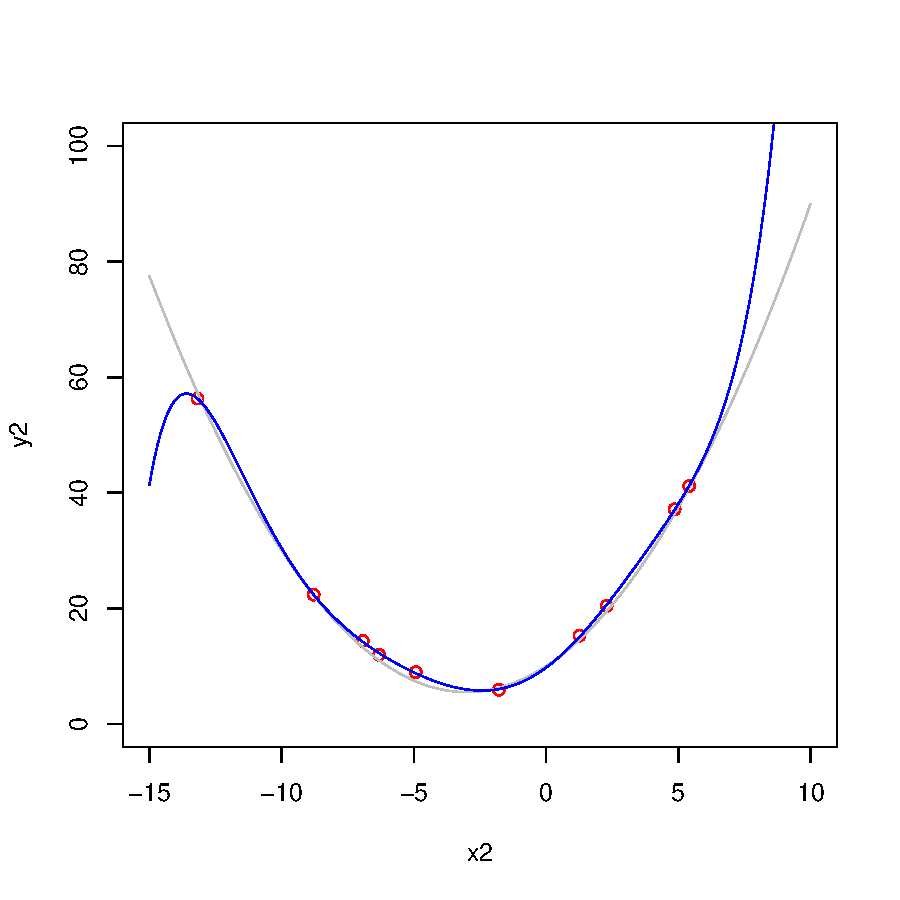
\includegraphics{aproximacao_polinomial-008}

\newpage
\subsection{Polinômio Grau 8 - 10 amostras}

\begin{Schunk}
\begin{Sinput}
>   N<-10
>   x<-runif(n=N, min=xmin,max=xmax)
>   xgrid<-seq(xmin,xmax,xstep)
>   yr<-(a1*x^2+a2*x+a3)+rnorm(length(x))
>   ygrid<-(a1*xgrid^2+a2*xgrid+a3)
>   plot(x,yr,col='red',type='p', xlim=c(xmin,xmax), ylim=c(ymin,ymax),xlab='',ylab='')
>   par(new=T)
>   plot(xgrid,ygrid,col='gray',type='l', xlim=c(xmin,xmax), ylim=c(ymin,ymax),xlab='',ylab='')
>   par(new=T)
>   #aproximacao de grau 7
>   H<-cbind(x^8,x^7,x^6,x^5,x^4,x^3,x^2,x,1)
>   w<-pseudoinverse(H) %*% yr
>   Hgrid<-cbind(xgrid^8,xgrid^7,xgrid^6,xgrid^5,xgrid^4,xgrid^3,xgrid^2,xgrid,1)
>   yhat<-H%*%w
>   yhatgrid<-Hgrid%*%w
>   plot(xgrid,yhatgrid,col='blue',type='l', xlim=c(xmin,xmax), ylim=c(ymin,ymax),xlab='x2',ylab='y2')
\end{Sinput}
\end{Schunk}
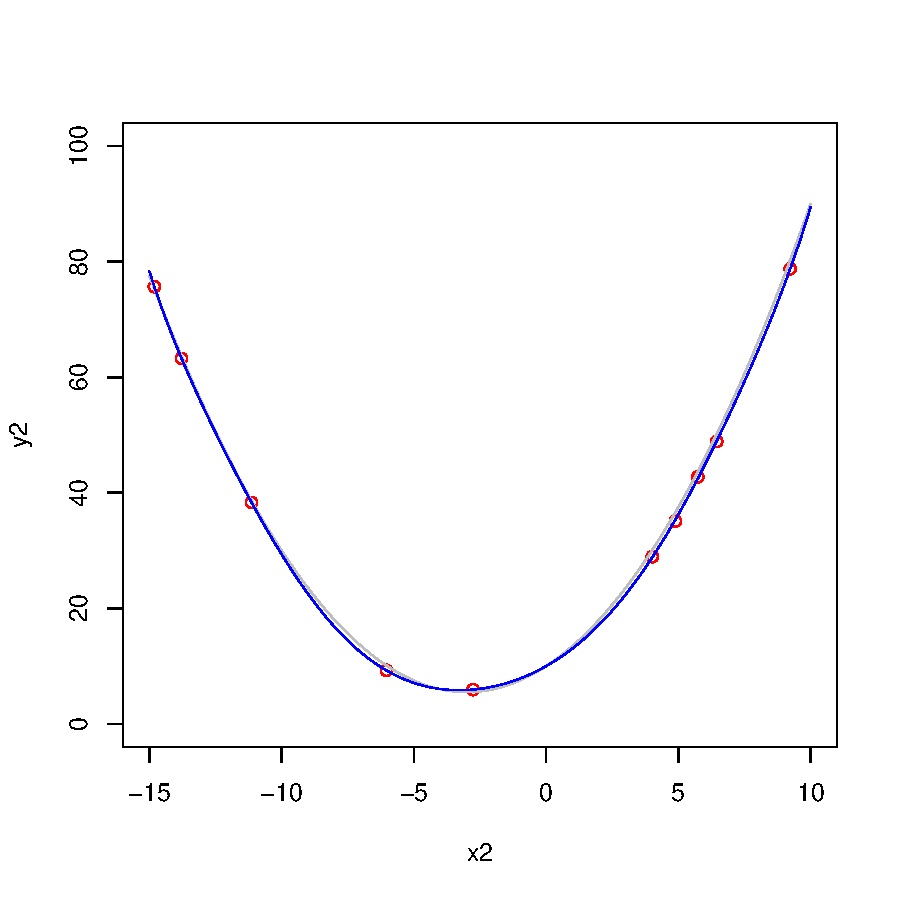
\includegraphics{aproximacao_polinomial-009}

\newpage
\section{Overfitting e Underfitting}

\begin{enumerate}
  \item \emph{Underfitting} ocorreu no polinômio de grau 1.
  \item \emph{Overfitting} occorreu nos polinômios de grau 7 e 8, principalmente no de grau 8.
\end{enumerate}

\newpage
\section{Aproximação Polinomial - 100 amostras}

\subsection{Polinômio Grau 1 - 100 amostras}

\begin{Schunk}
\begin{Sinput}
>   N<-100
>   x<-runif(n=N, min=xmin,max=xmax)
>   xgrid<-seq(xmin,xmax,xstep)
>   yr<-(a1*x^2+a2*x+a3)+rnorm(length(x))
>   ygrid<-(a1*xgrid^2+a2*xgrid+a3)
>   plot(x,yr,col='red',type='p', xlim=c(xmin,xmax), ylim=c(ymin,ymax),xlab='',ylab='')
>   par(new=T)
>   plot(xgrid,ygrid,col='gray',type='l', xlim=c(xmin,xmax), ylim=c(ymin,ymax),xlab='',ylab='')
>   par(new=T)
>   #aproximacao de grau 1
>   H<-cbind(x,1)
>   w<-pseudoinverse(H) %*% yr
>   Hgrid<-cbind(xgrid,1)
>   yhat<-H%*%w
>   yhatgrid<-Hgrid%*%w
>   plot(xgrid,yhatgrid,col='blue',type='l', xlim=c(xmin,xmax), ylim=c(ymin,ymax),xlab='x',ylab='y')
\end{Sinput}
\end{Schunk}
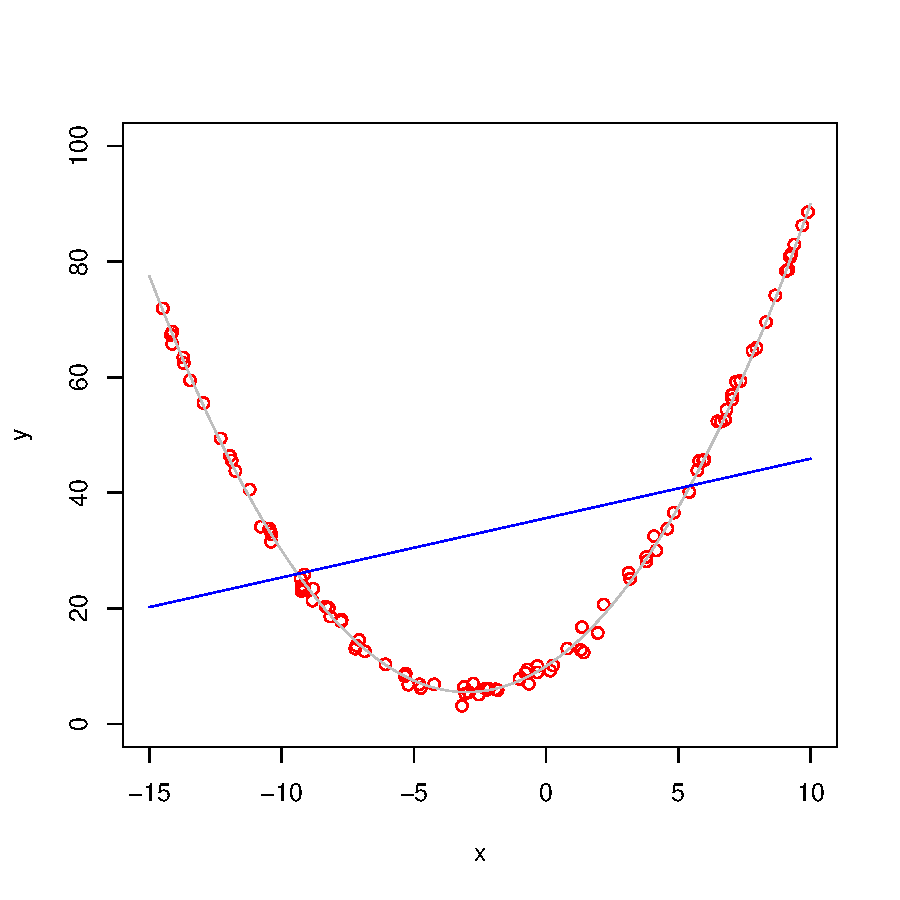
\includegraphics{aproximacao_polinomial-010}

\newpage
\subsection{Polinômio Grau 2 - 100 amostras}

\begin{Schunk}
\begin{Sinput}
>   N<-100
>   x<-runif(n=N, min=xmin,max=xmax)
>   xgrid<-seq(xmin,xmax,xstep)
>   yr<-(a1*x^2+a2*x+a3)+rnorm(length(x))
>   ygrid<-(a1*xgrid^2+a2*xgrid+a3)
>   plot(x,yr,col='red',type='p', xlim=c(xmin,xmax), ylim=c(ymin,ymax),xlab='',ylab='')
>   par(new=T)
>   plot(xgrid,ygrid,col='gray',type='l', xlim=c(xmin,xmax), ylim=c(ymin,ymax),xlab='',ylab='')
>   par(new=T)
>   #aproximacao de grau 2
>   H<-cbind(x^2,x,1)
>   w<-pseudoinverse(H) %*% yr
>   Hgrid<-cbind(xgrid^2,xgrid,1)
>   yhat<-H%*%w
>   yhatgrid<-Hgrid%*%w
>   plot(xgrid,yhatgrid,col='blue',type='l', xlim=c(xmin,xmax), ylim=c(ymin,ymax),xlab='x',ylab='y')
\end{Sinput}
\end{Schunk}
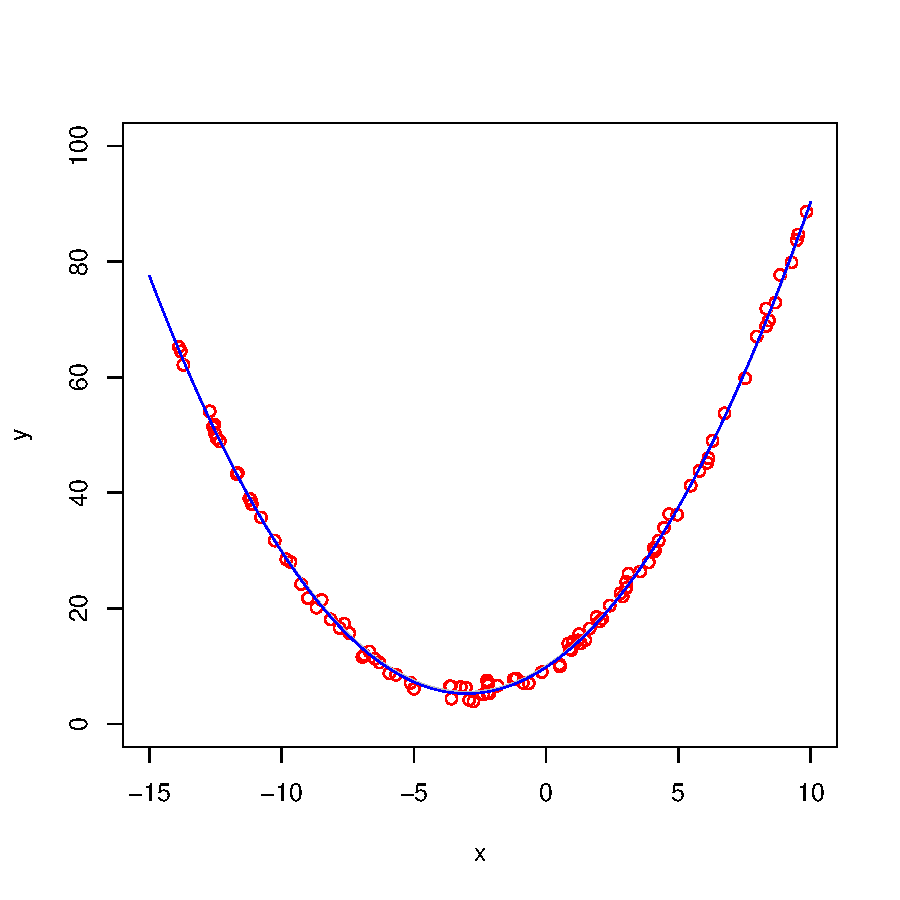
\includegraphics{aproximacao_polinomial-011}

\newpage
\subsection{Polinômio Grau 3 - 100 amostras}

\begin{Schunk}
\begin{Sinput}
>   N<-100
>   x<-runif(n=N, min=xmin,max=xmax)
>   xgrid<-seq(xmin,xmax,xstep)
>   yr<-(a1*x^2+a2*x+a3)+rnorm(length(x))
>   ygrid<-(a1*xgrid^2+a2*xgrid+a3)
>   plot(x,yr,col='red',type='p', xlim=c(xmin,xmax), ylim=c(ymin,ymax),xlab='',ylab='')
>   par(new=T)
>   plot(xgrid,ygrid,col='gray',type='l', xlim=c(xmin,xmax), ylim=c(ymin,ymax),xlab='',ylab='')
>   par(new=T)
>   #aproximacao de grau 3
>   H<-cbind(x^3,x^2,x,1)
>   w<-pseudoinverse(H) %*% yr
>   Hgrid<-cbind(xgrid^3,xgrid^2,xgrid,1)
>   yhat<-H%*%w
>   yhatgrid<-Hgrid%*%w
>   plot(xgrid,yhatgrid,col='blue',type='l', xlim=c(xmin,xmax), ylim=c(ymin,ymax),xlab='x',ylab='y')
\end{Sinput}
\end{Schunk}
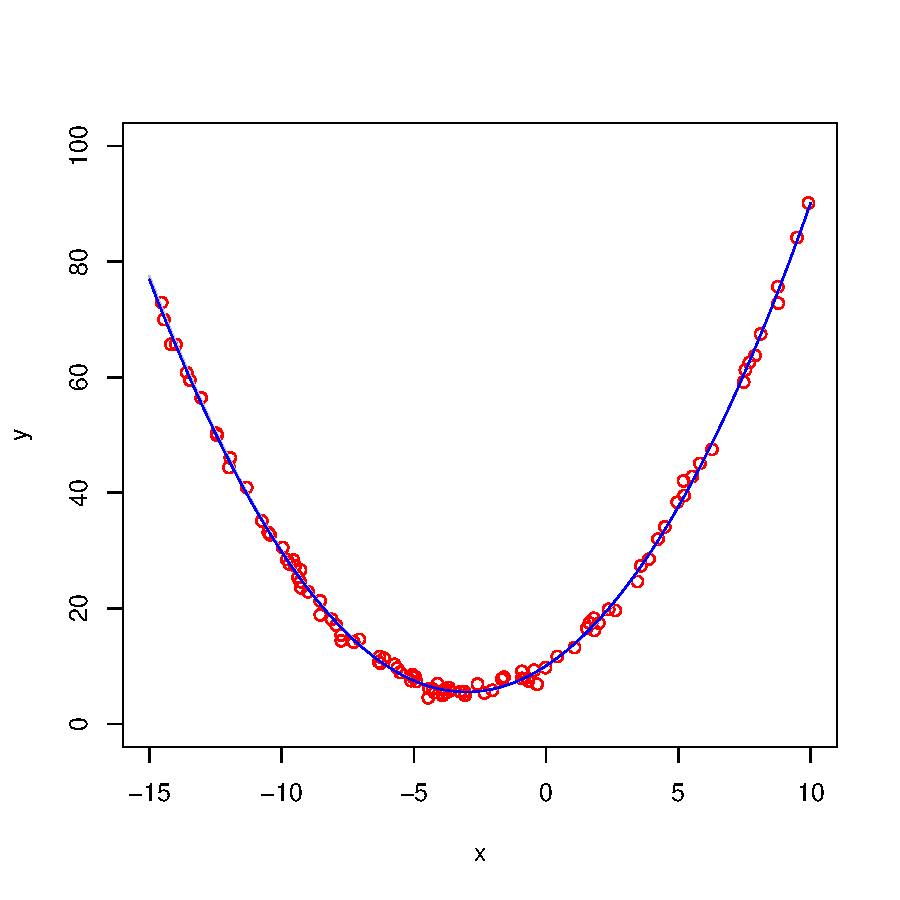
\includegraphics{aproximacao_polinomial-012}

\newpage
\subsection{Polinômio Grau 4 - 100 amostras}

\begin{Schunk}
\begin{Sinput}
>   N<-100
>   x<-runif(n=N, min=xmin,max=xmax)
>   xgrid<-seq(xmin,xmax,xstep)
>   yr<-(a1*x^2+a2*x+a3)+rnorm(length(x))
>   ygrid<-(a1*xgrid^2+a2*xgrid+a3)
>   plot(x,yr,col='red',type='p', xlim=c(xmin,xmax), ylim=c(ymin,ymax),xlab='',ylab='')
>   par(new=T)
>   plot(xgrid,ygrid,col='gray',type='l', xlim=c(xmin,xmax), ylim=c(ymin,ymax),xlab='',ylab='')
>   par(new=T)
>   #aproximacao de grau 4
>   H<-cbind(x^4,x^3,x^2,x,1)
>   w<-pseudoinverse(H) %*% yr
>   Hgrid<-cbind(xgrid^4,xgrid^3,xgrid^2,xgrid,1)
>   yhat<-H%*%w
>   yhatgrid<-Hgrid%*%w
>   plot(xgrid,yhatgrid,col='blue',type='l', xlim=c(xmin,xmax), ylim=c(ymin,ymax),xlab='x2',ylab='y2')
\end{Sinput}
\end{Schunk}
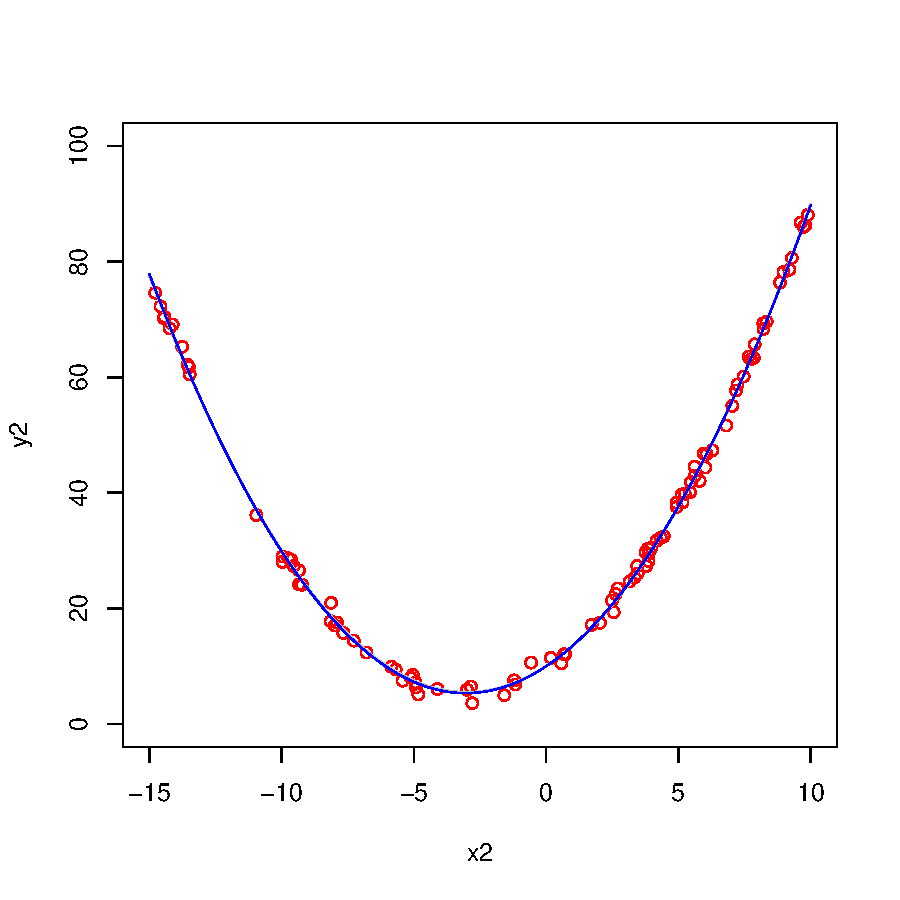
\includegraphics{aproximacao_polinomial-013}

\newpage
\subsection{Polinômio Grau 5 - 100 amostras}

\begin{Schunk}
\begin{Sinput}
>   N<-100
>   x<-runif(n=N, min=xmin,max=xmax)
>   xgrid<-seq(xmin,xmax,xstep)
>   yr<-(a1*x^2+a2*x+a3)+rnorm(length(x))
>   ygrid<-(a1*xgrid^2+a2*xgrid+a3)
>   plot(x,yr,col='red',type='p', xlim=c(xmin,xmax), ylim=c(ymin,ymax),xlab='',ylab='')
>   par(new=T)
>   plot(xgrid,ygrid,col='gray',type='l', xlim=c(xmin,xmax), ylim=c(ymin,ymax),xlab='',ylab='')
>   par(new=T)
>   #aproximacao de grau 5
>   H<-cbind(x^5,x^4,x^3,x^2,x,1)
>   w<-pseudoinverse(H) %*% yr
>   Hgrid<-cbind(xgrid^5,xgrid^4,xgrid^3,xgrid^2,xgrid,1)
>   yhat<-H%*%w
>   yhatgrid<-Hgrid%*%w
>   plot(xgrid,yhatgrid,col='blue',type='l', xlim=c(xmin,xmax), ylim=c(ymin,ymax),xlab='x2',ylab='y2')
\end{Sinput}
\end{Schunk}
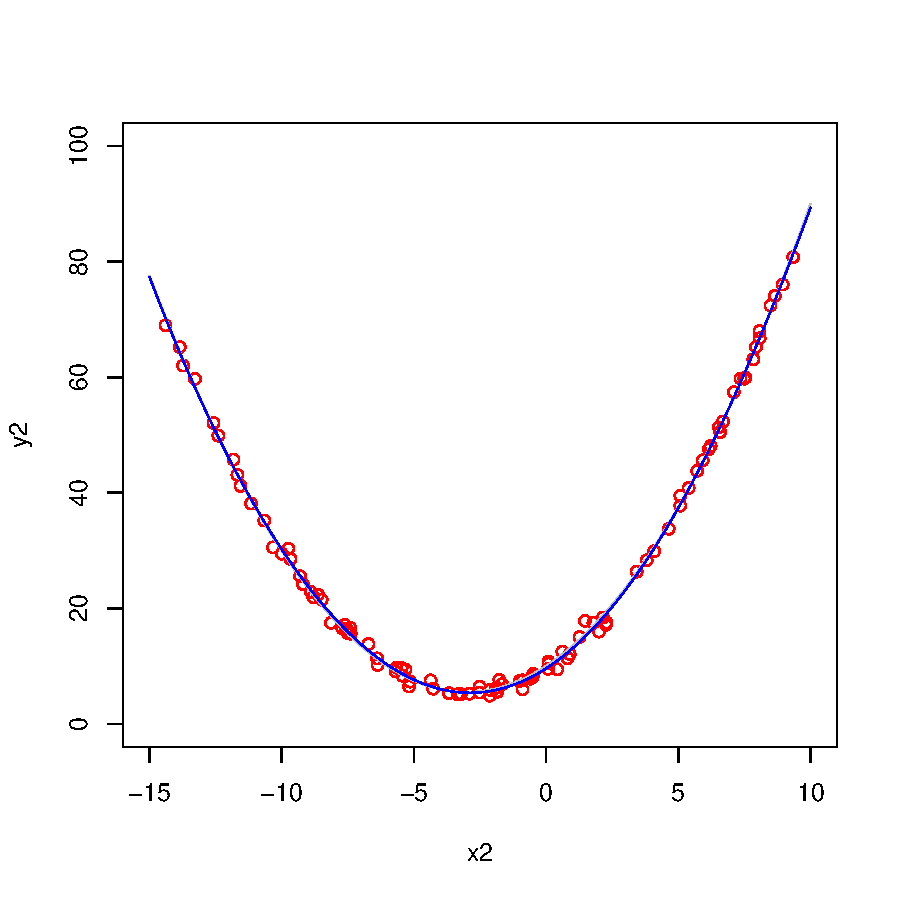
\includegraphics{aproximacao_polinomial-014}

\newpage
\subsection{Polinômio Grau 6 - 100 amostras}

\begin{Schunk}
\begin{Sinput}
>   N<-100
>   x<-runif(n=N, min=xmin,max=xmax)
>   xgrid<-seq(xmin,xmax,xstep)
>   yr<-(a1*x^2+a2*x+a3)+rnorm(length(x))
>   ygrid<-(a1*xgrid^2+a2*xgrid+a3)
>   plot(x,yr,col='red',type='p', xlim=c(xmin,xmax), ylim=c(ymin,ymax),xlab='',ylab='')
>   par(new=T)
>   plot(xgrid,ygrid,col='gray',type='l', xlim=c(xmin,xmax), ylim=c(ymin,ymax),xlab='',ylab='')
>   par(new=T)
>   #aproximacao de grau 6
>   H<-cbind(x^6,x^5,x^4,x^3,x^2,x,1)
>   w<-pseudoinverse(H) %*% yr
>   Hgrid<-cbind(xgrid^6,xgrid^5,xgrid^4,xgrid^3,xgrid^2,xgrid,1)
>   yhat<-H%*%w
>   yhatgrid<-Hgrid%*%w
>   plot(xgrid,yhatgrid,col='blue',type='l', xlim=c(xmin,xmax), ylim=c(ymin,ymax),xlab='x2',ylab='y2')
\end{Sinput}
\end{Schunk}
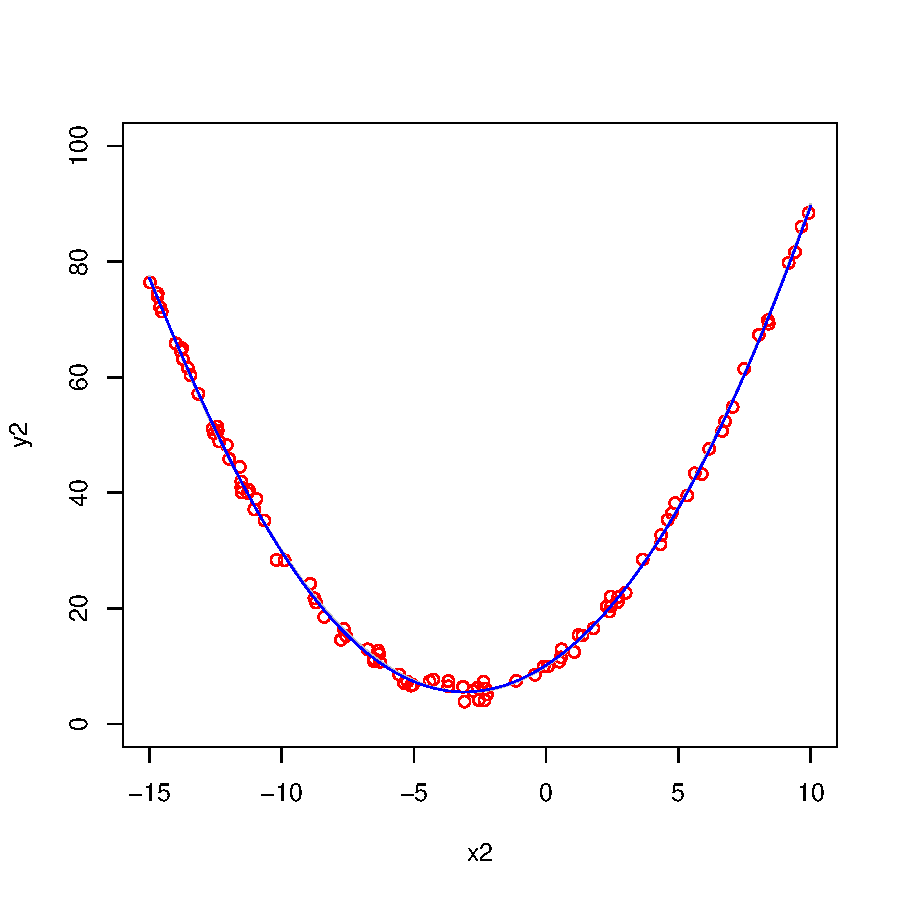
\includegraphics{aproximacao_polinomial-015}

\newpage
\subsection{Polinômio Grau 7 - 100 amostras}

\begin{Schunk}
\begin{Sinput}
>   N<-100
>   x<-runif(n=N, min=xmin,max=xmax)
>   xgrid<-seq(xmin,xmax,xstep)
>   yr<-(a1*x^2+a2*x+a3)+rnorm(length(x))
>   ygrid<-(a1*xgrid^2+a2*xgrid+a3)
>   plot(x,yr,col='red',type='p', xlim=c(xmin,xmax), ylim=c(ymin,ymax),xlab='',ylab='')
>   par(new=T)
>   plot(xgrid,ygrid,col='gray',type='l', xlim=c(xmin,xmax), ylim=c(ymin,ymax),xlab='',ylab='')
>   par(new=T)
>   #aproximacao de grau 7
>   H<-cbind(x^7,x^6,x^5,x^4,x^3,x^2,x,1)
>   w<-pseudoinverse(H) %*% yr
>   Hgrid<-cbind(xgrid^7,xgrid^6,xgrid^5,xgrid^4,xgrid^3,xgrid^2,xgrid,1)
>   yhat<-H%*%w
>   yhatgrid<-Hgrid%*%w
>   plot(xgrid,yhatgrid,col='blue',type='l', xlim=c(xmin,xmax), ylim=c(ymin,ymax),xlab='x2',ylab='y2')
\end{Sinput}
\end{Schunk}
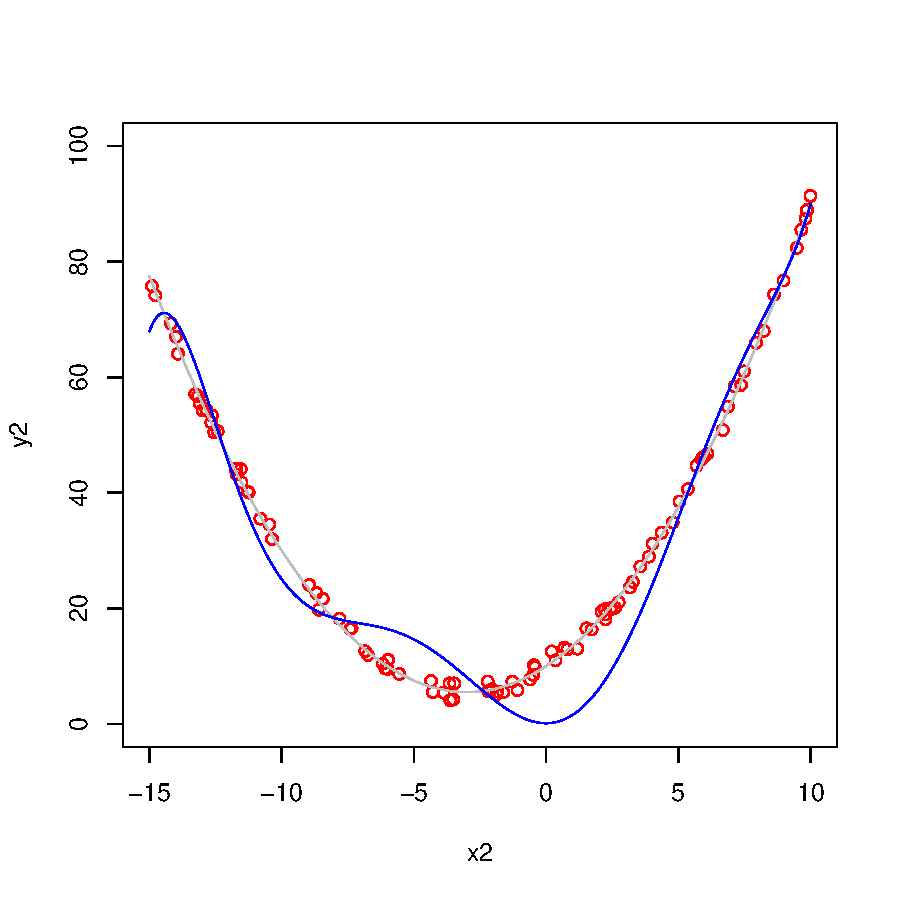
\includegraphics{aproximacao_polinomial-016}

\newpage
\subsection{Polinômio Grau 8 - 100 amostras}

\begin{Schunk}
\begin{Sinput}
>   N<-100
>   x<-runif(n=N, min=xmin,max=xmax)
>   xgrid<-seq(xmin,xmax,xstep)
>   yr<-(a1*x^2+a2*x+a3)+rnorm(length(x))
>   ygrid<-(a1*xgrid^2+a2*xgrid+a3)
>   plot(x,yr,col='red',type='p', xlim=c(xmin,xmax), ylim=c(ymin,ymax),xlab='',ylab='')
>   par(new=T)
>   plot(xgrid,ygrid,col='gray',type='l', xlim=c(xmin,xmax), ylim=c(ymin,ymax),xlab='',ylab='')
>   par(new=T)
>   #aproximacao de grau 7
>   H<-cbind(x^8,x^7,x^6,x^5,x^4,x^3,x^2,x,1)
>   w<-pseudoinverse(H) %*% yr
>   Hgrid<-cbind(xgrid^8,xgrid^7,xgrid^6,xgrid^5,xgrid^4,xgrid^3,xgrid^2,xgrid,1)
>   yhat<-H%*%w
>   yhatgrid<-Hgrid%*%w
>   plot(xgrid,yhatgrid,col='blue',type='l', xlim=c(xmin,xmax), ylim=c(ymin,ymax),xlab='x2',ylab='y2')
\end{Sinput}
\end{Schunk}
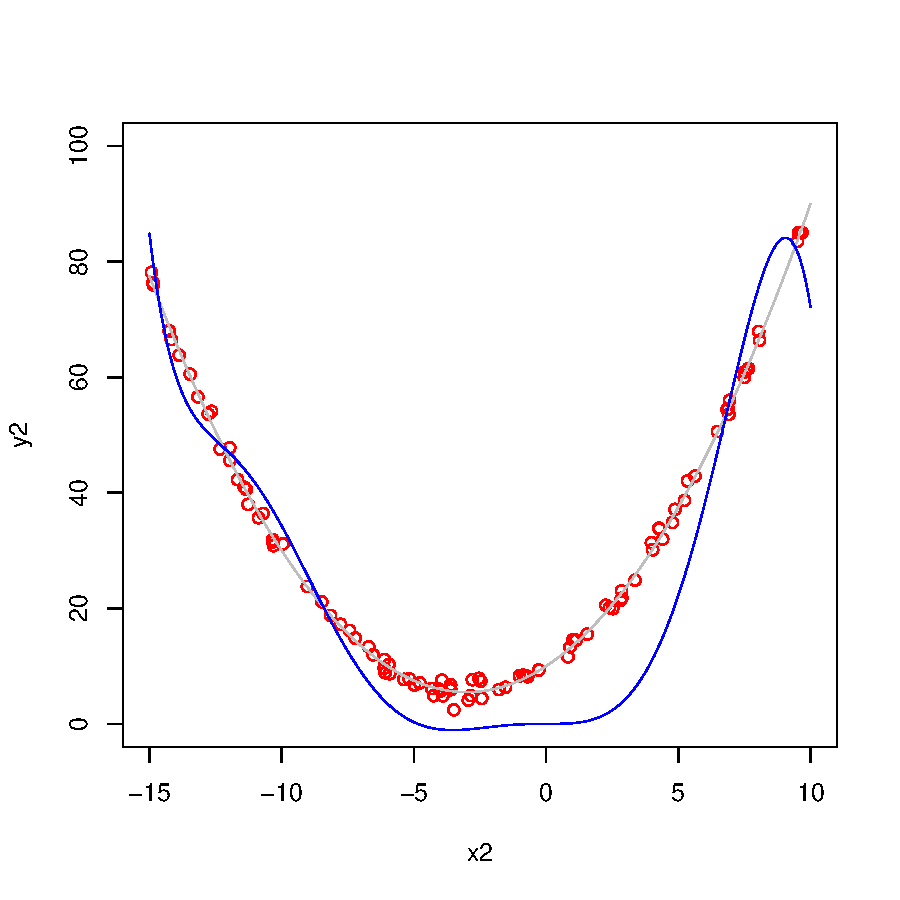
\includegraphics{aproximacao_polinomial-017}


\newpage
\section{Aproximadores Polinomiais e Redes Neurais Artificiais}

Enquanto a aproximação polinomial pode ser representada pela equação matricial:

$$ \bm{w} = \bm{H^+} \bm{y} $$

Uma Rede Neural Artificial pode ser representada pela equação:

$$f(\texttt{x},\texttt{z}_1,...,\texttt{z}_p,w_1,...,w_p) = \phi (\sum_{i=1}^{p}h_i(\texttt{x},\texttt{z}_i)w_i + \beta)$$

\end{document}
